\documentclass{article}
\usepackage{hyperref}
\usepackage{algorithm2e}
\usepackage{graphicx}
\usepackage{amsmath}
\usepackage{amssymb}
\hypersetup{
    colorlinks=true,
    linkcolor=magenta,
    urlcolor=blue
    }
\urlstyle{same}
\graphicspath{ {./images/} }
\RestyleAlgo{ruled}
\SetKwComment{Comment}{/* }{ */}

\title{AMS 326-1: Exam 3}
\author{
Numerical Analysis, Spring 2025 \\
Author: Joe Martinez \\
SBU ID: 112416928
}
\date{April 29, 2025}


\begin{document}

\maketitle

All of the problems solved were done in Python, with the use of the random, math, shapely, numpy, and mathplotlib libraries.

\section{Problem 2: Buffon's Needles on a Quadrifolium}
Given the quadrifolium expressed in polar coordinates as $r=sin(2\theta)$, and a box $[-1, -1]\times [1, 1]$ enclosing it, our goal was find the probability of tossing randomly tossed needles of varying length crossing our "rose" or quadrifolium curve. If a needle crossed the curve twice, it was only counted once. Our approach to simulate this was to run a Monte Carlo simulation with 444444 needle with the list of varying lengths being
\[
    L=\frac{1}{10}\text{, } \frac{1}{5}\text{, } \frac{1}{4}\text{, } \frac{1}{3}\text{, } \frac{1}{2}\text{, } \frac{1}{1}
\]


Being a Monte Carlo simulation, we randomly sampled x and y values for each needle a uniform distribution in the range of $[-1,1]$, given the box enclosing the curve to represent the center of the needle. For the orientation of the needle, we sampled an angle from a unfirom distribution in the range of $[0, 2\pi]$. Having the angle and the length of the needle, we create a line that represented the needle by addding and subtracting the distance from the center of the needle to its endpoints. This was done by as shown below, where $\theta$ represents the angle and $l$ represents the length of the needle:

\[\Delta x = \frac{l}{2}cos(\theta)\]
\[\Delta y = \frac{l}{2}sin(\theta)\]
\[\text{Line: } [(x - \Delta x, y - \Delta y), (x + \Delta x, y + \Delta y)]\]

Each needle and the "rose" curve were presenteded using hte LineString object in the Shapely Python library. The code to generate the rose curve can be seen in Figure \ref{fig:rose}. Using the \textit{shapely::intersection(curve1 ,curve2)} function, we found if a given needle intersected the "rose" curve. We would count the number of needles that cross the curve and divide this by the total number of needles generated, producing our probability for a given length. This was done for each length. The algorithm for calculating the probability given a length of a needle is in Figure \ref{fig:alg}.

\begin{figure}[hbt!]
    \centering
    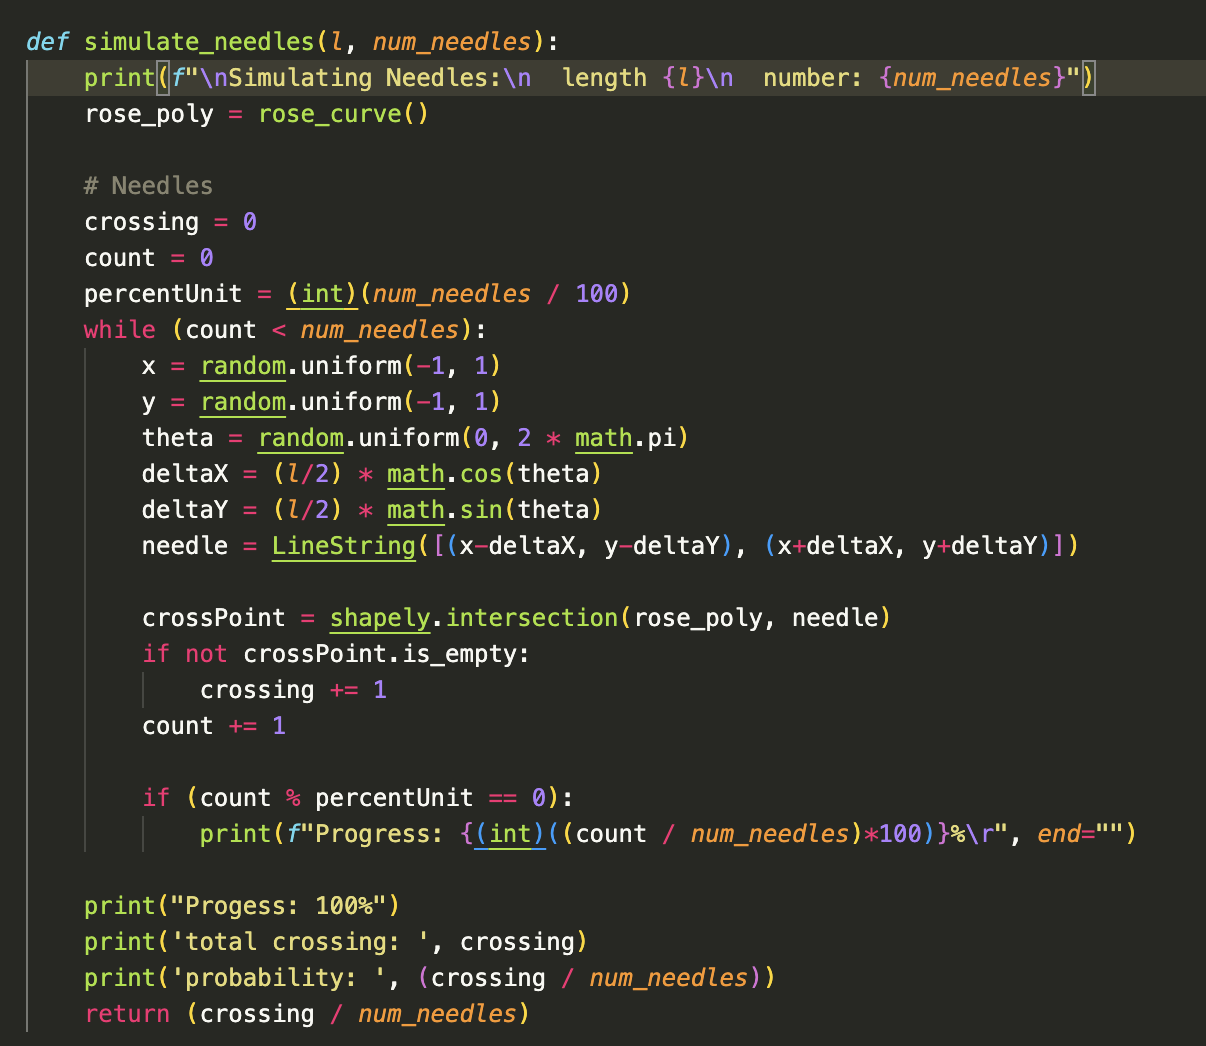
\includegraphics[width=0.95\linewidth]{images/alg.png}
    \caption{PDF of crossing 0 lines based on disk diameter}
    \label{fig:alg}
\end{figure}
\begin{figure}[hbt!]
    \centering
    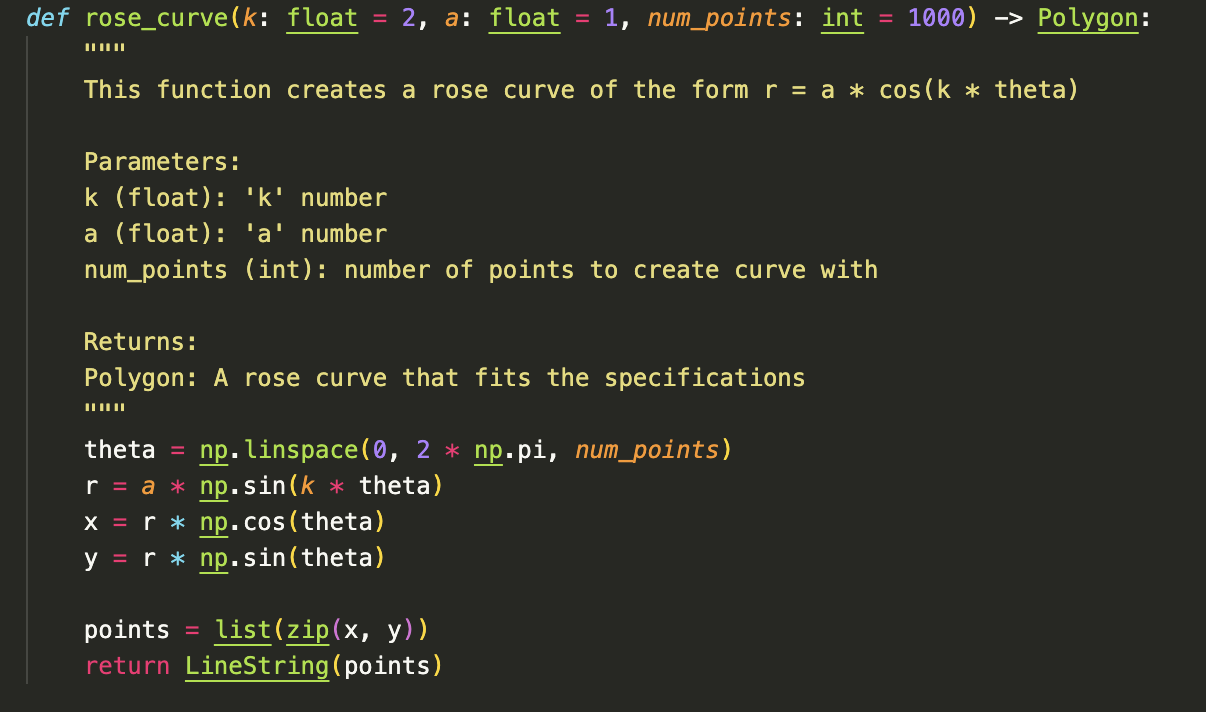
\includegraphics[width=0.95\linewidth]{images/rose.png}
    \caption{PDF of crossing 0 lines based on disk diameter}
    \label{fig:rose}
\end{figure}


The following are the probabilities we found
\begin{table}
    \centering
    \begin{tabular}{|c|c|}
        \hline
        Needle Length & Probability of Crossing \\
        \hline \hline
        $0.1$ & 0.1416 \\
        \hline
        $0.2$ & 0.2725 \\
        \hline
        $0.25$ & 0.3341 \\
        \hline
        $\frac{1}{3}$ & 0.4307 \\
        \hline
        $0.5$ & 0.6031 \\
        \hline
        $1$ & 0.7972 \\
        \hline


    \end{tabular}
\end{table}



\end{document}